\documentclass{loyola-beamer}
\renewcommand{\titlelogo}{logo/luc-rev.svg}
\renewcommand{\slidelogo}{logo/luc.svg}
\usepackage{physics}
\usepackage{graphicx}
\usepackage{hyperref}


\title{Mobile Phone Detector based on Op Amp}
% \subtitle{Made with Beamer}
\author{Alfaifi, Ammar}
\institute{KFUPM}
\renewcommand{\slidefoot}{Department of Physics - PHYS308}

\begin{document}

\begin{titleframe}{}
	\maketitle
\end{titleframe}

\begin{frame}{Contents}
	\tableofcontents
\end{frame}


% Start of the slides

\begin{titleframe}{Introduction}
	Concept and Background
\end{titleframe}

\section{What's all about?}

\begin{frame}{Problem}
	
\includegraphics[width=0.5\textwidth]{../mobile-not-allowed.jpg}
	\begin{itemize}
		\item Mobile phones are great tools, but they are bnned in some places.
		\item Detecting phones being around is important.
		\item Providing  easy-to-use tools to detect phones.
	\end{itemize}
\end{frame}

\begin{frame}{What's Being Detected ?}
	\begin{block}{Key Point}
		Almost all mobile phones emit EM radiation.
	\end{block}

	GSM, 2G, Searching for network, or SMS $\sim$ 800 MHz

	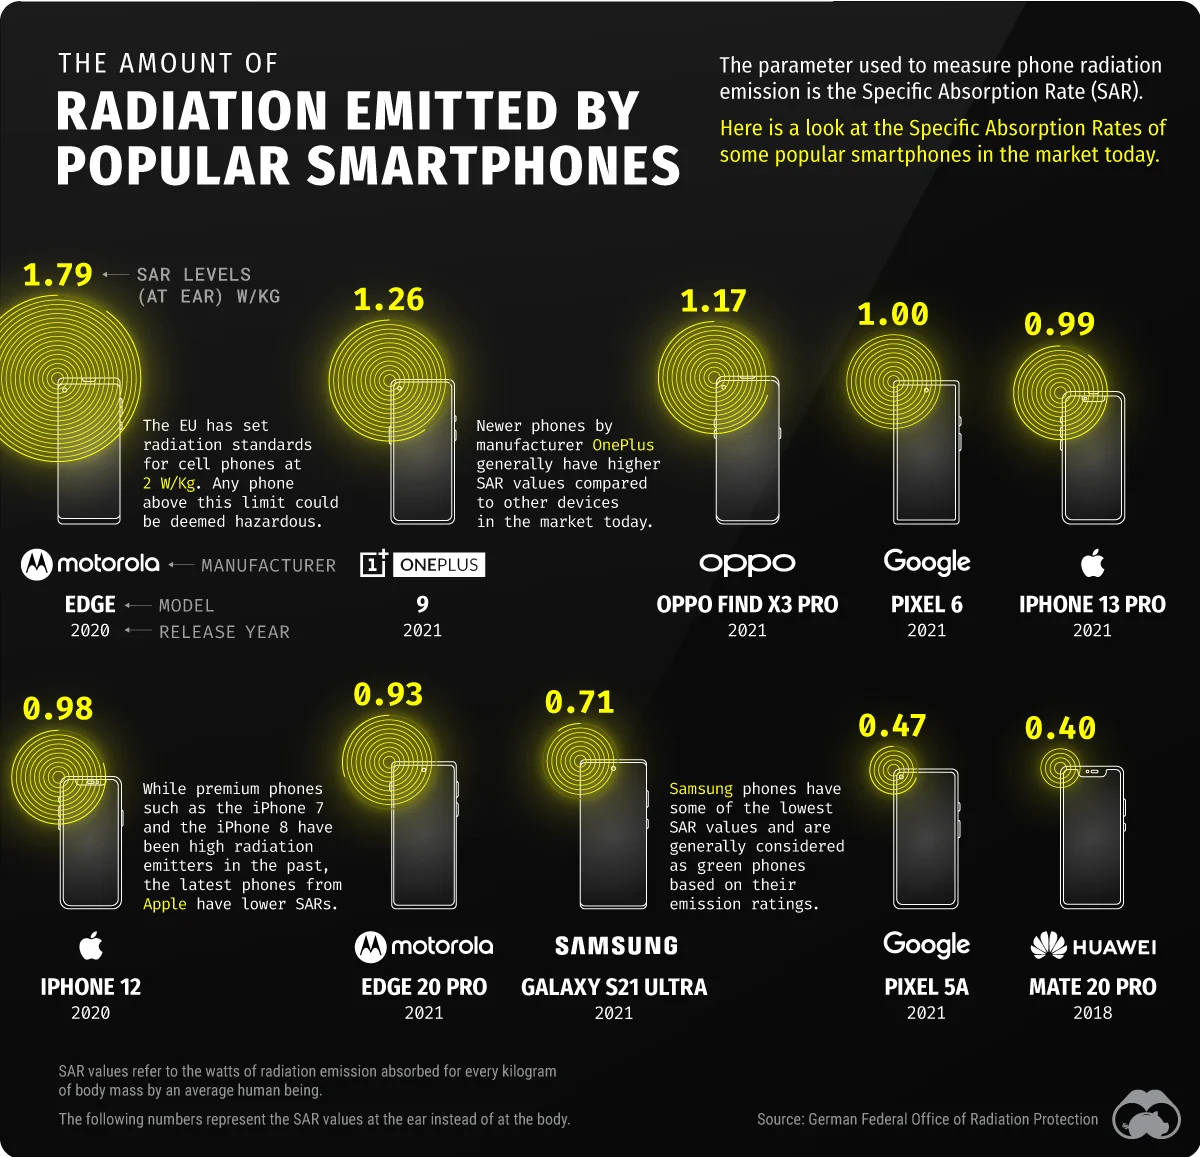
\includegraphics[width=0.5\textwidth]{../Radiation.jpg}
\end{frame}

\section{Design \& Implementaion}

\begin{frame}{Cicuit Diagram}
	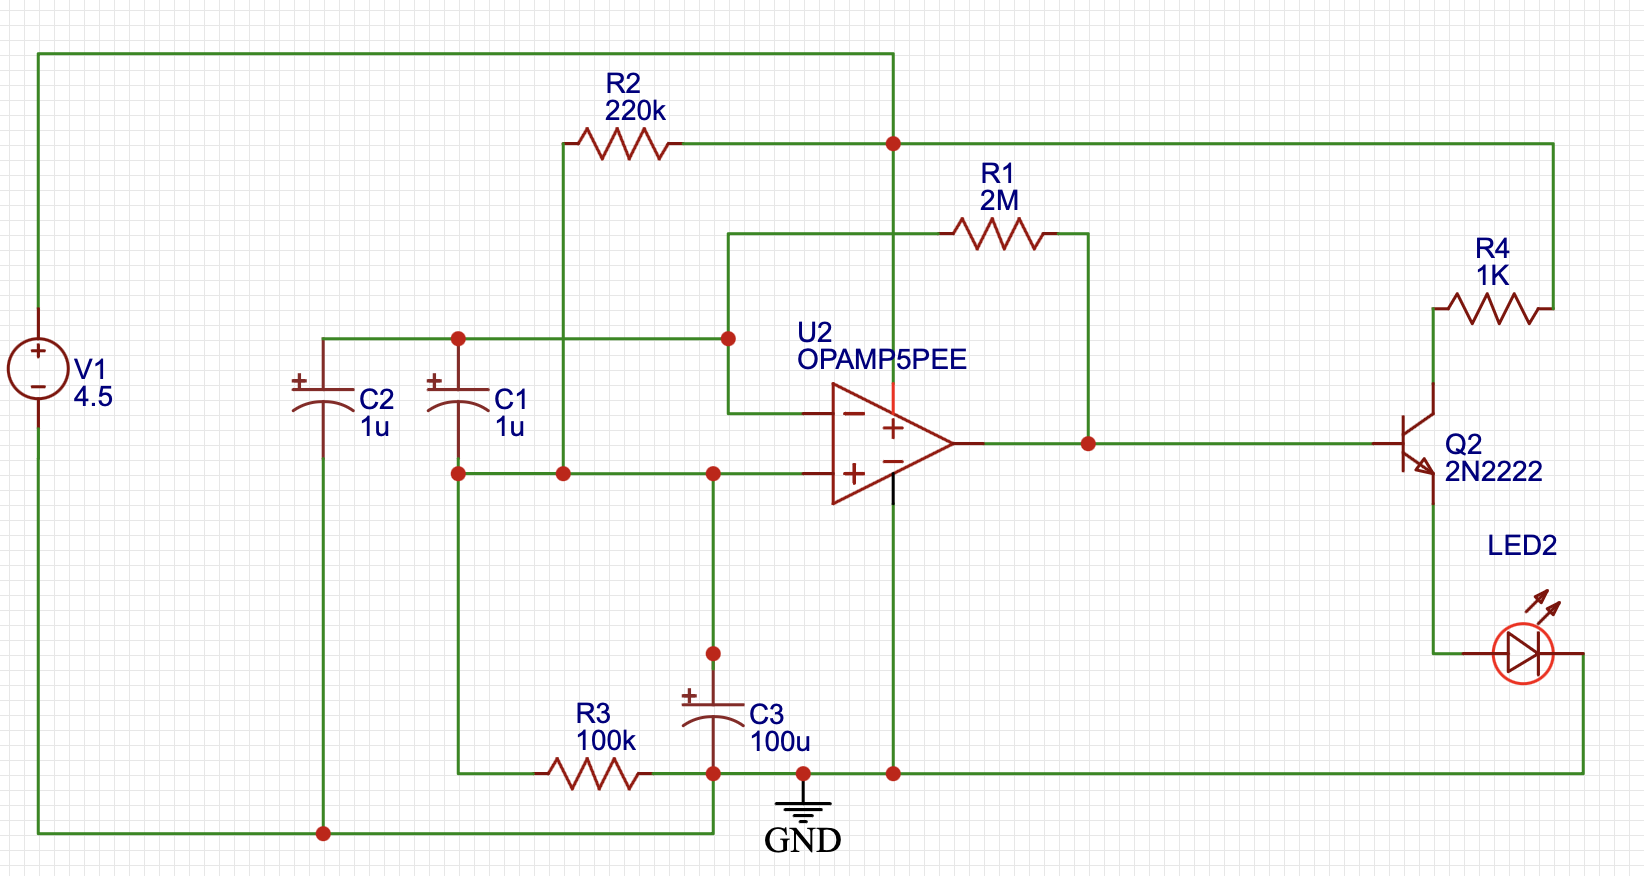
\includegraphics[width=0.9\textwidth]{../detector-circuit.png}

	\begin{itemize}
		\item LM358P Op Amp
		\item NPN Transistor
		\item LED \& Buzzer
		\item Capacitros and resistors
	\end{itemize}
\end{frame}


\begin{frame}{In-Lab Testing}
	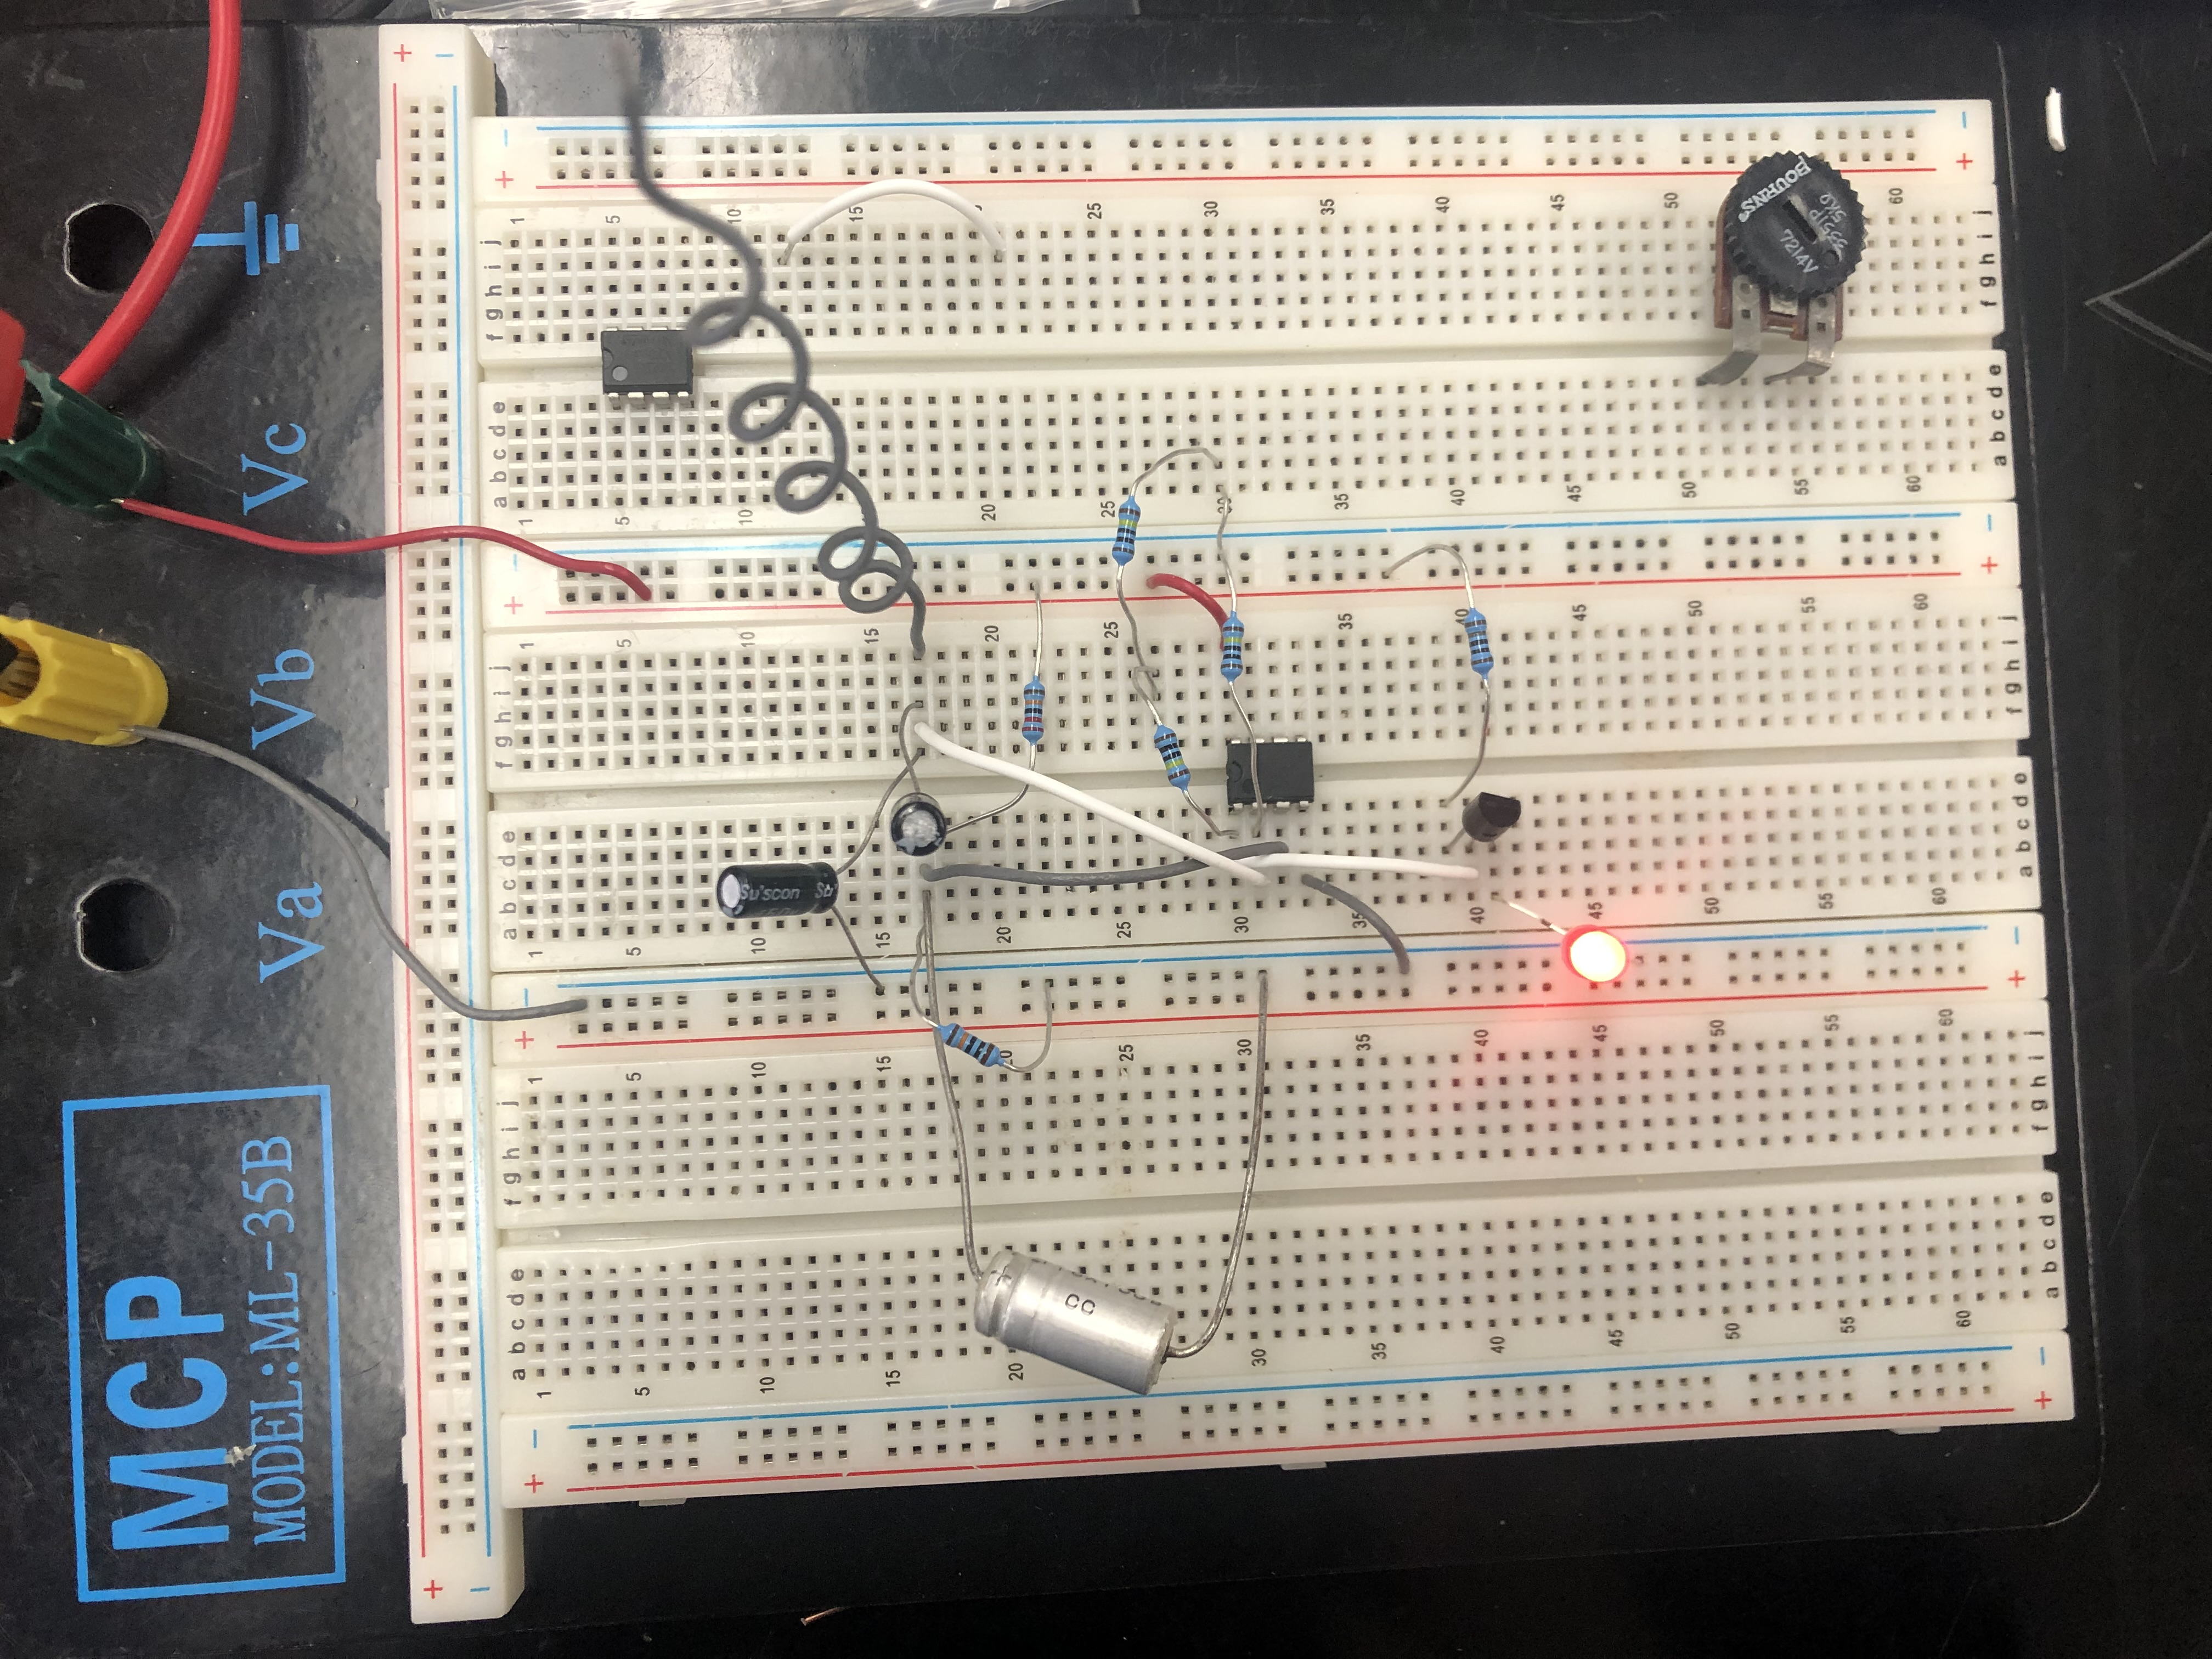
\includegraphics[width=0.9\textwidth]{../breadboard.jpeg}
\end{frame}


\begin{titleframe}{A Quick Demo}
\end{titleframe}

\section{Limitations}

\begin{frame}{Limitations}
	\begin{itemize}
		\item Very small coverage circle.
		\item Requires antenna, and more tuning for is.
		\item Radiation-free workplace.
		\item Such circuits cannot be simulated.
	\end{itemize}
\end{frame}

\section{What's Next ?}

\begin{frame}{What's Next ?}
	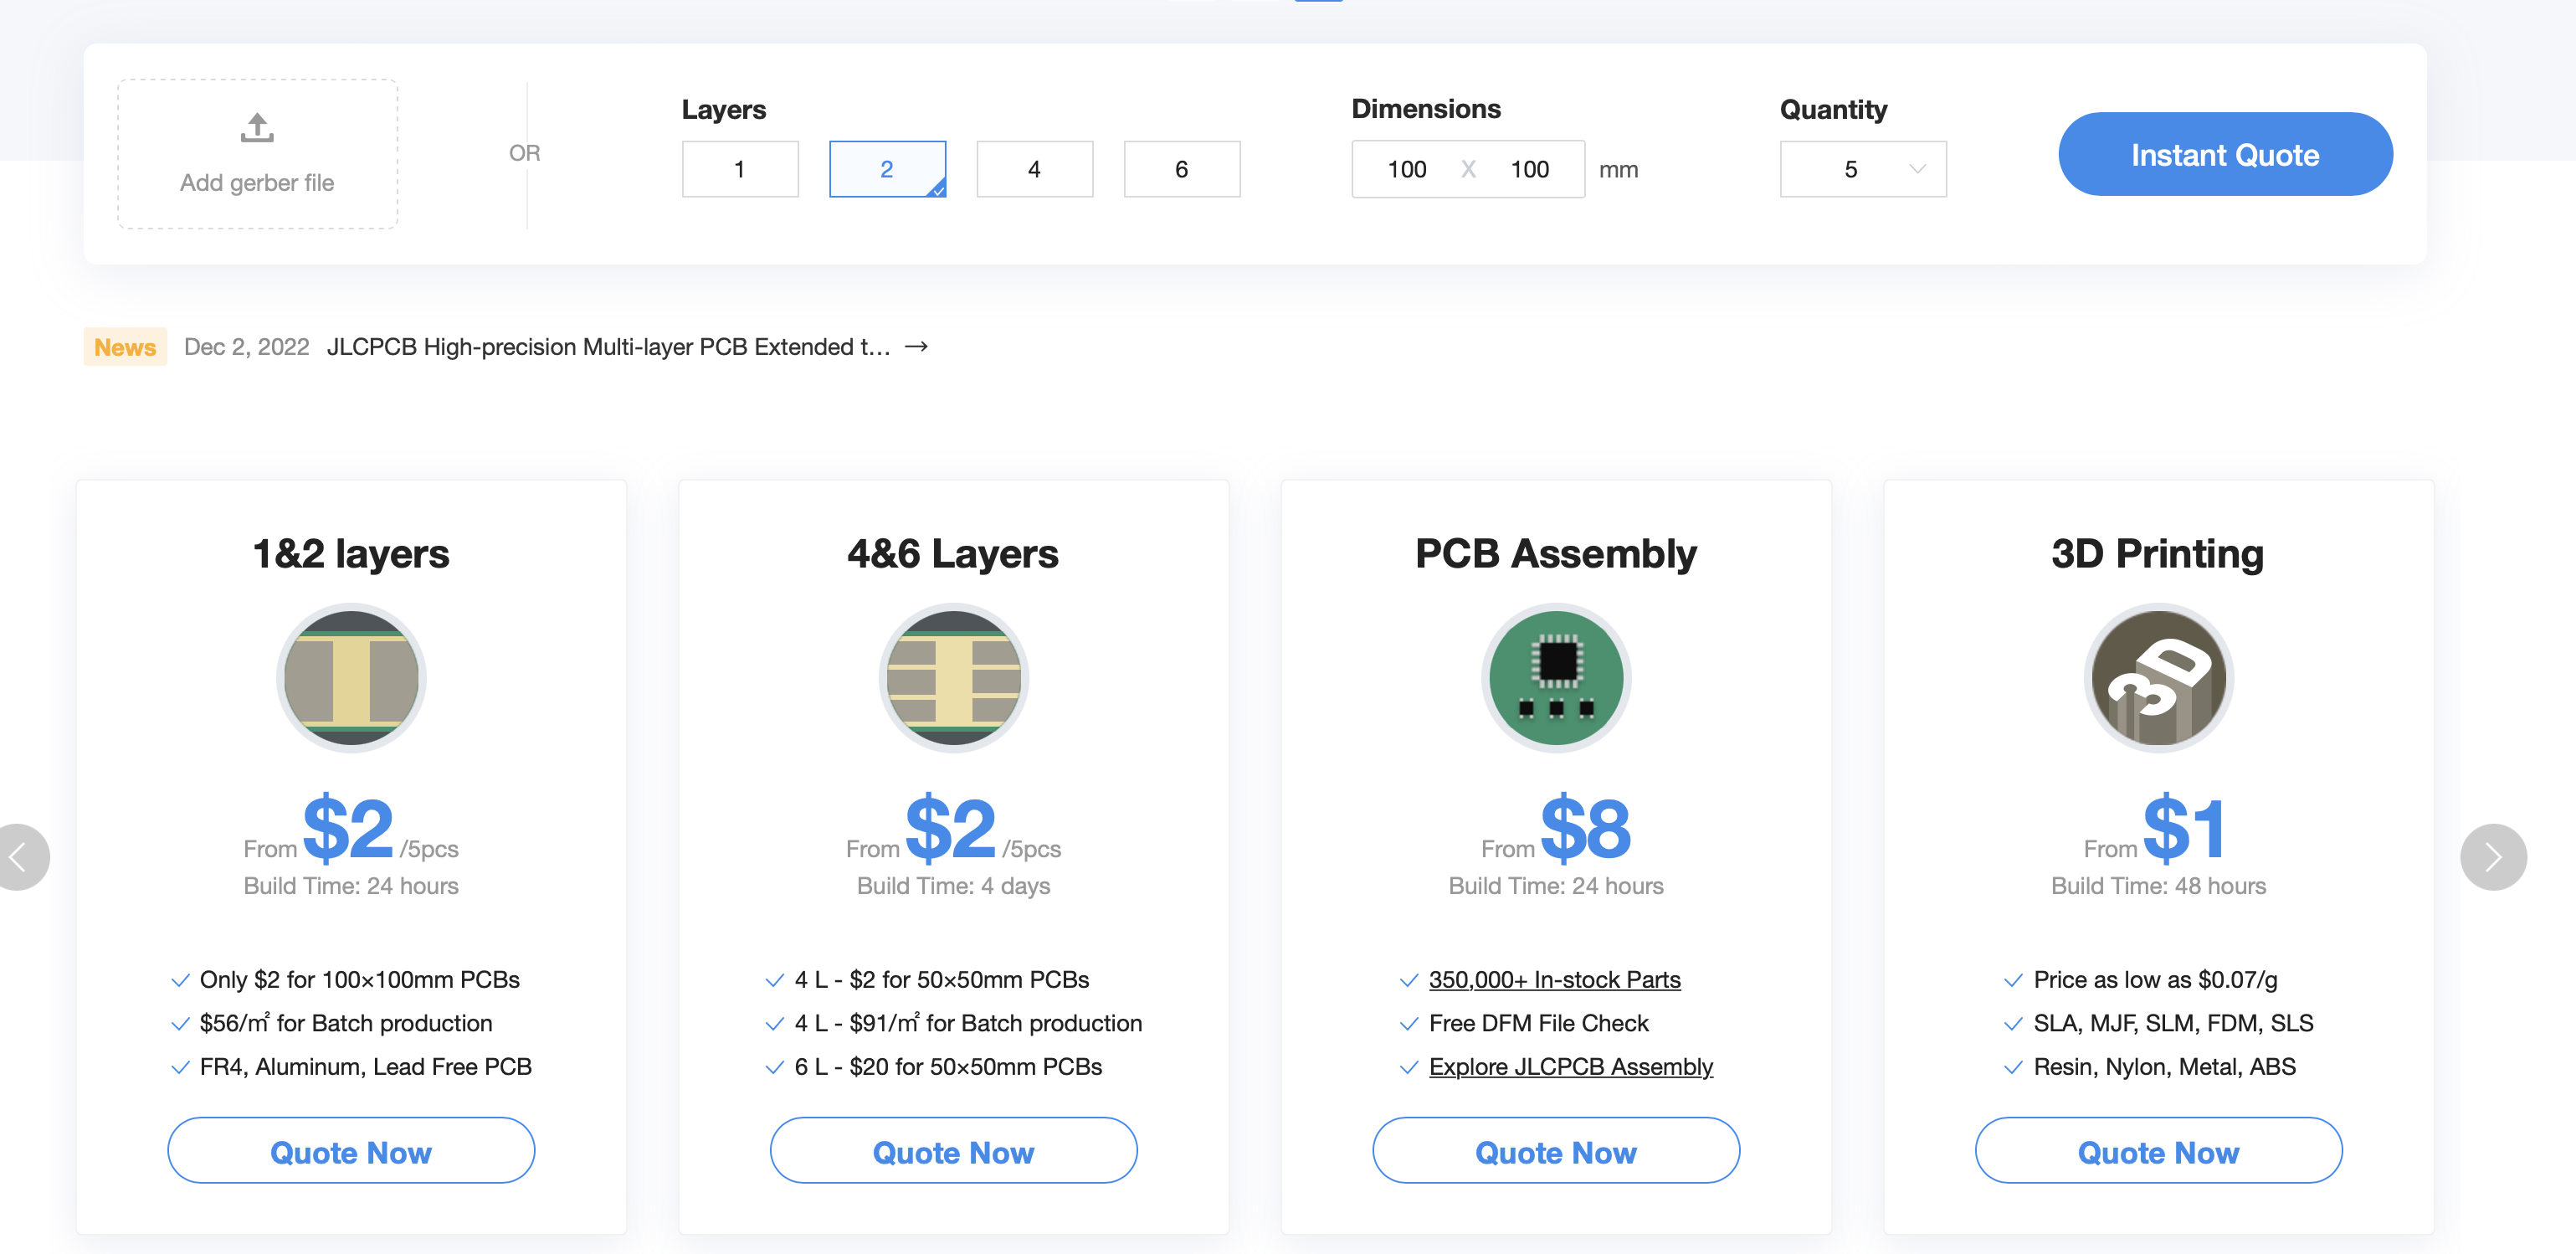
\includegraphics[width=0.8\textwidth]{../PCB-printer.png}
\end{frame}

\begin{frame}{PCB Before Routing}
	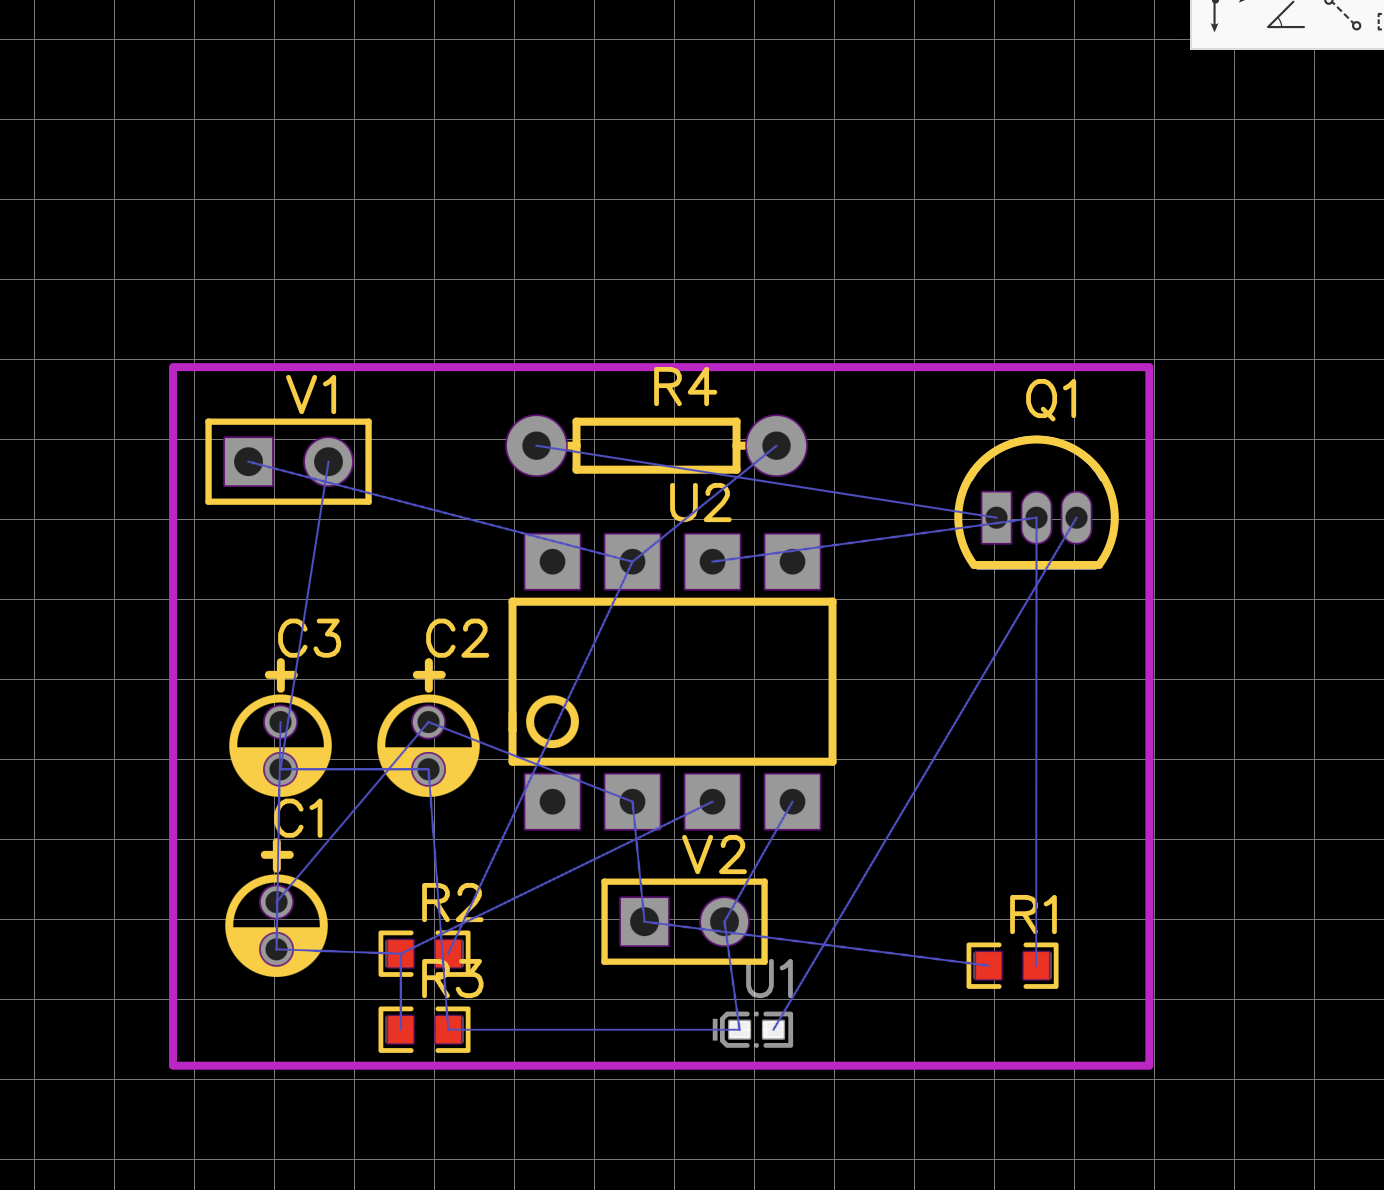
\includegraphics[width=0.8\textwidth]{../PCB-before.png}
\end{frame}


\begin{frame}{PCB After Routing}
	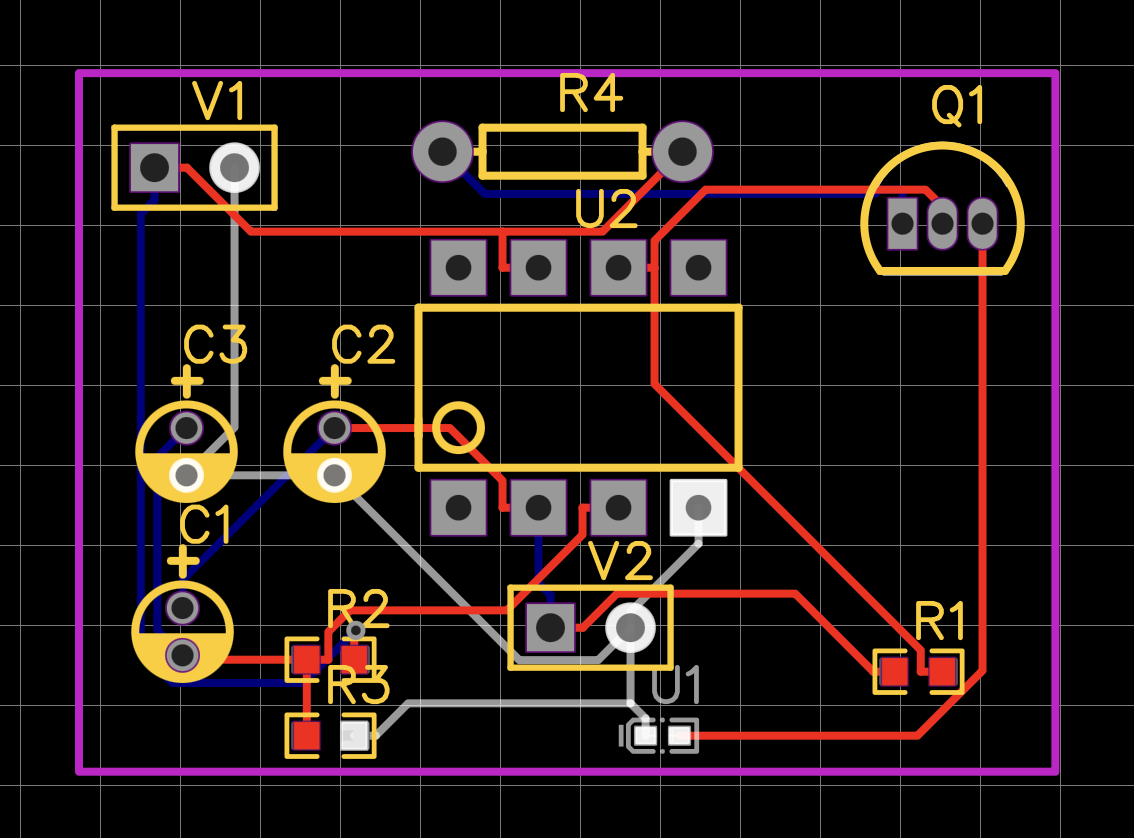
\includegraphics[width=0.8\textwidth]{../PCB-after.png}
\end{frame}


\begin{frame}{3D View}
	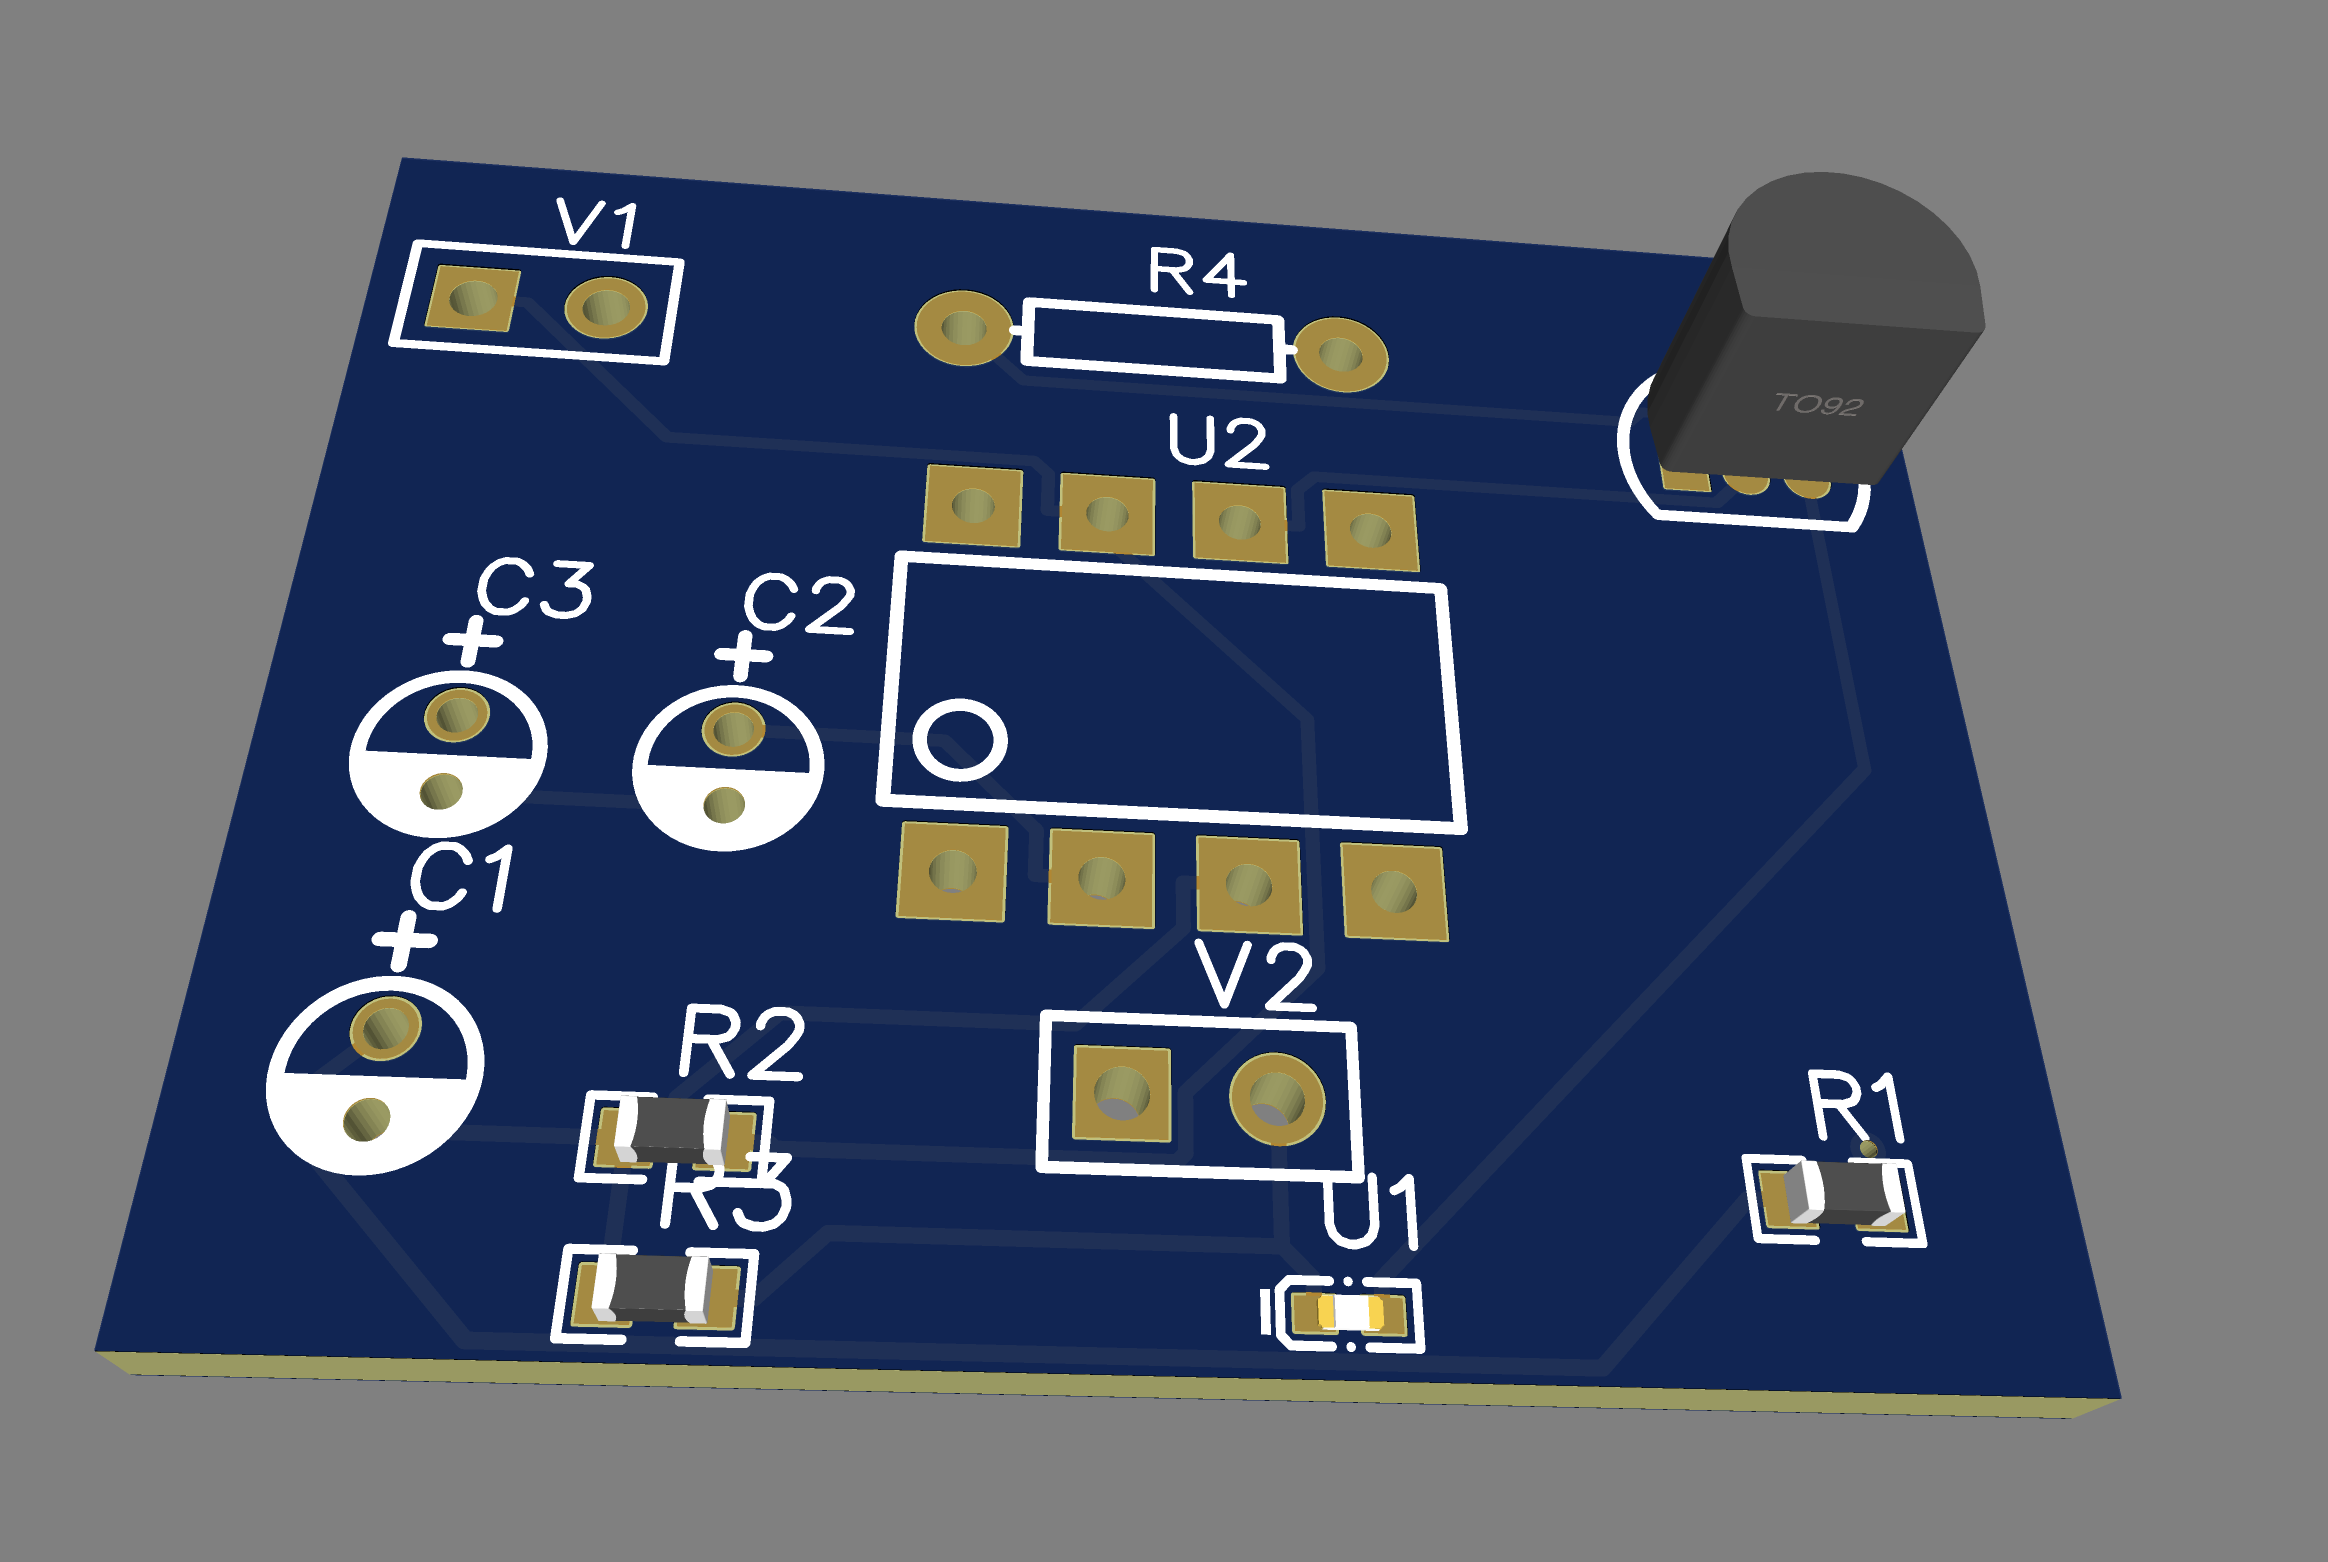
\includegraphics[width=0.8\textwidth]{../3D-PCB.png}
\end{frame}


\begin{frame}{Conclusion}

	The mobile phone detector based on an op amp is an effective and low-cost project,
	to deletct the existing of a mobile phone around via EM radiation emitted by the GSM signals.

\end{frame}





\begin{titleframe}{Thank you for listening!}

\end{titleframe}

\end{document}
